% Options for packages loaded elsewhere
\PassOptionsToPackage{unicode}{hyperref}
\PassOptionsToPackage{hyphens}{url}
%
\documentclass[
  english,
  man, donotrepeattitle,floatsintext]{apa6}
\usepackage{lmodern}
\usepackage{amssymb,amsmath}
\usepackage{ifxetex,ifluatex}
\ifnum 0\ifxetex 1\fi\ifluatex 1\fi=0 % if pdftex
  \usepackage[T1]{fontenc}
  \usepackage[utf8]{inputenc}
  \usepackage{textcomp} % provide euro and other symbols
\else % if luatex or xetex
  \usepackage{unicode-math}
  \defaultfontfeatures{Scale=MatchLowercase}
  \defaultfontfeatures[\rmfamily]{Ligatures=TeX,Scale=1}
\fi
% Use upquote if available, for straight quotes in verbatim environments
\IfFileExists{upquote.sty}{\usepackage{upquote}}{}
\IfFileExists{microtype.sty}{% use microtype if available
  \usepackage[]{microtype}
  \UseMicrotypeSet[protrusion]{basicmath} % disable protrusion for tt fonts
}{}
\makeatletter
\@ifundefined{KOMAClassName}{% if non-KOMA class
  \IfFileExists{parskip.sty}{%
    \usepackage{parskip}
  }{% else
    \setlength{\parindent}{0pt}
    \setlength{\parskip}{6pt plus 2pt minus 1pt}}
}{% if KOMA class
  \KOMAoptions{parskip=half}}
\makeatother
\usepackage{xcolor}
\IfFileExists{xurl.sty}{\usepackage{xurl}}{} % add URL line breaks if available
\IfFileExists{bookmark.sty}{\usepackage{bookmark}}{\usepackage{hyperref}}
\hypersetup{
  pdflang={en-EN},
  pdfkeywords={UK Biobank; Occupational factors; Work; Employment; fMRI; rsMRI; Interoception; Inflammation; Cytokine; Immune function.},
  hidelinks,
  pdfcreator={LaTeX via pandoc}}
\urlstyle{same} % disable monospaced font for URLs
\usepackage{graphicx}
\makeatletter
\def\maxwidth{\ifdim\Gin@nat@width>\linewidth\linewidth\else\Gin@nat@width\fi}
\def\maxheight{\ifdim\Gin@nat@height>\textheight\textheight\else\Gin@nat@height\fi}
\makeatother
% Scale images if necessary, so that they will not overflow the page
% margins by default, and it is still possible to overwrite the defaults
% using explicit options in \includegraphics[width, height, ...]{}
\setkeys{Gin}{width=\maxwidth,height=\maxheight,keepaspectratio}
% Set default figure placement to htbp
\makeatletter
\def\fps@figure{htbp}
\makeatother
\setlength{\emergencystretch}{3em} % prevent overfull lines
\providecommand{\tightlist}{%
  \setlength{\itemsep}{0pt}\setlength{\parskip}{0pt}}
\setcounter{secnumdepth}{-\maxdimen} % remove section numbering
% Make \paragraph and \subparagraph free-standing
\ifx\paragraph\undefined\else
  \let\oldparagraph\paragraph
  \renewcommand{\paragraph}[1]{\oldparagraph{#1}\mbox{}}
\fi
\ifx\subparagraph\undefined\else
  \let\oldsubparagraph\subparagraph
  \renewcommand{\subparagraph}[1]{\oldsubparagraph{#1}\mbox{}}
\fi
% Manuscript styling
\usepackage{upgreek}
\captionsetup{font=singlespacing,justification=justified}

% Table formatting
\usepackage{longtable}
\usepackage{lscape}
% \usepackage[counterclockwise]{rotating}   % Landscape page setup for large tables
\usepackage{multirow}		% Table styling
\usepackage{tabularx}		% Control Column width
\usepackage[flushleft]{threeparttable}	% Allows for three part tables with a specified notes section
\usepackage{threeparttablex}            % Lets threeparttable work with longtable

% Create new environments so endfloat can handle them
% \newenvironment{ltable}
%   {\begin{landscape}\begin{center}\begin{threeparttable}}
%   {\end{threeparttable}\end{center}\end{landscape}}
\newenvironment{lltable}{\begin{landscape}\begin{center}\begin{ThreePartTable}}{\end{ThreePartTable}\end{center}\end{landscape}}

% Enables adjusting longtable caption width to table width
% Solution found at http://golatex.de/longtable-mit-caption-so-breit-wie-die-tabelle-t15767.html
\makeatletter
\newcommand\LastLTentrywidth{1em}
\newlength\longtablewidth
\setlength{\longtablewidth}{1in}
\newcommand{\getlongtablewidth}{\begingroup \ifcsname LT@\roman{LT@tables}\endcsname \global\longtablewidth=0pt \renewcommand{\LT@entry}[2]{\global\advance\longtablewidth by ##2\relax\gdef\LastLTentrywidth{##2}}\@nameuse{LT@\roman{LT@tables}} \fi \endgroup}

% \setlength{\parindent}{0.5in}
% \setlength{\parskip}{0pt plus 0pt minus 0pt}

% \usepackage{etoolbox}
\makeatletter
\patchcmd{\HyOrg@maketitle}
  {\section{\normalfont\normalsize\abstractname}}
  {\section*{\normalfont\normalsize\abstractname}}
  {}{\typeout{Failed to patch abstract.}}
\makeatother
\shorttitle{Pre-registration: Neural markers of occupational wellbeing}
\author{Raul Ungureanu\textsuperscript{1, 2}\ \& Charlotte Rae\textsuperscript{2,3}}
\affiliation{
\vspace{0.5cm}
\textsuperscript{1} Sussex Neuroscience, School of Life Sciences, University of Sussex, Falmer, UK\\\textsuperscript{2} School of Psychology, University of Sussex, Falmer, UK\\\textsuperscript{3} Sackler Centre for Consciousness Science, University of Sussex, Falmer, UK}
\authornote{

Correspondence concerning this article should be addressed to Raul Ungureanu, School of Psychology, University of Sussex, Falmer, BN1 9QH. E-mail: r.ungureanu@sussex.ac.uk}
\keywords{UK Biobank; Occupational factors; Work; Employment; fMRI; rsMRI; Interoception; Inflammation; Cytokine; Immune function.\newline\indent Word count: X}
\DeclareDelayedFloatFlavor{ThreePartTable}{table}
\DeclareDelayedFloatFlavor{lltable}{table}
\DeclareDelayedFloatFlavor*{longtable}{table}
\makeatletter
\renewcommand{\efloat@iwrite}[1]{\immediate\expandafter\protected@write\csname efloat@post#1\endcsname{}}
\makeatother
\usepackage{csquotes}
\usepackage{fancyhdr}
\pagestyle{fancy}
\fancyhf{}
\fancyhead[L]{\bfseries Pre-registration $\colon$ Neural markers of occupational wellbeing.}
\thispagestyle{empty}
\fancyhead[R]{\thepage}
\renewcommand{\footrulewidth}{0.4pt}
\renewcommand{\headrulewidth}{0.2pt}
\ifxetex
  % Load polyglossia as late as possible: uses bidi with RTL langages (e.g. Hebrew, Arabic)
  \usepackage{polyglossia}
  \setmainlanguage[]{english}
\else
  \usepackage[shorthands=off,main=english]{babel}
\fi
\newlength{\cslhangindent}
\setlength{\cslhangindent}{1.5em}
\newenvironment{cslreferences}%
  {\setlength{\parindent}{0pt}%
  \everypar{\setlength{\hangindent}{\cslhangindent}}\ignorespaces}%
  {\par}

\title{\textbf{Pre-registration:}\\
\textbf{Characterising the neural markers of occupational wellbeing.}}

\date{}

\abstract{
Occupational factors can have numerous impacts on wellbeing and mental health, from under- or over-employment, to shift work, and commuting time.
However, the neural mechanisms by which such occupational factors influence subjective wellbeing, and engender vulnerability to mental health symptoms, are less well understood. This project aims to characterize the neurophysiological processes through which occupational factors affect our health and wellbeing in an analysis of data from the UK Biobank: a large-scale epidemiological study of 500,000 individuals, \textasciitilde40,000 of whom have completed an MRI session at time of writing.
To characterise neural markers of occupational wellbeing in the Biobank, we will implement a multifactorial analysis strategy, beginning with an exploratory analysis of the non-imaging variables in our dataset. This will allow us to sufficiently characterise the association of occupational factors with sociodemographic, lifestyle, and health-related information in order to appropriately control for these in subsequent analyses focusing on neurophysiology.
We intend to successively update our preregistration documentation as we proceed through each analysis step in this project. This document forms the first document in this series. Analysis workflows, together with time-stamped logs detailing data access events, if available, will be linked to subsequent preregistration documentation.
}

\begin{document}
\maketitle

\newpage

\hypertarget{background}{%
\subsection{Background}\label{background}}

Work takes up a huge chunk of our adult lives: the average Briton works approximately \(42\) hours per week,\textsuperscript{{[}1{]}} with an additional \textasciitilde4.9 hours spent on commuting,\textsuperscript{{[}2{]}} and an estimate of \textasciitilde10.1 hours in unpaid overtime.\textsuperscript{{[}3{]}} These numbers have been growing in the past 30 years\textsuperscript{{[}1--3{]}} without benefits to productivity. Importantly, a growing body of evidence suggests a strong negative impact on our health and wellbeing. Long working hours are associated with a higher risk of cardiovascular disease,\textsuperscript{{[}4{]}} higher incidence of depressive,\textsuperscript{{[}5{]}} and anxiety symptoms,\textsuperscript{{[}4{]}} deficient cognitive function,\textsuperscript{{[}6{]}} and adverse physiological changes.\textsuperscript{{[}7{]}} Moreover, interventional studies show that a reduction in working hours benefits both health and productivity.\textsuperscript{{[}8,9{]}} However, we do not yet understand the neurobiological implications of our modern, increasingly intense, working patterns. Three reasons motivate the need for such an understanding:

\begin{itemize}
\item
  The brain acts as an interface between the body and the environment, therefore, it is key for grasping the mechanism through which occupational factors are affecting our health and wellbeing.
\item
  Without it we cannot ascertain the true short-term impact of working patterns on our cognitive function and physiological health, let alone the long-term, potentially irreversible, effects on our mental health and wellbeing.
\item
  Scientific evidence is needed to inform public policy and industry standards surrounding healthy work patterns.
\end{itemize}

\newpage

\hypertarget{aim-and-objectives}{%
\subsection{Aim and objectives}\label{aim-and-objectives}}

This project aims to characterize the neurophysiological processes through which work patterns and other occupational factors affect our health and wellbeing, with the following objectives:

\begin{itemize}
\tightlist
\item
  Identify occupational factors that have a meaningful impact on neuronal function and describe the mechanism of impact.
\item
  Assess how physiological inflammatory responses are altered by occupational factors.
\item
  Determine how the identified neuronal and inflammatory markers jointly affect our physical and mental health.
\end{itemize}

Progress against these objectives will help develop a holistic insight into why our wellbeing is affected by modern work patterns and other occupational factors.

\newpage

\hypertarget{rationale}{%
\subsection{Rationale}\label{rationale}}

The impact of working patterns on our neurophysiology is still not comprehensively understood; therefore our investigative plan does not build solely and directly on prior work in this specific arena. However, we have identified inadequate sleep as one principal means through which the influence of occupational factors on wellbeing is likely to manifest. First, relative to all other activities, work is the primary waking activity exchanged for sleep.\textsuperscript{{[}10{]}} Second, it is increasingly common for workers to accumulate sleep debt throughout the working week and attempt to catch-up on the weekend, a countermeasure that has been shown to often be ineffective in combating the deleterious effects of weekday sleep debt.\textsuperscript{{[}11--14{]}} Finally, working longer hours is associated with significantly reduced sleep duration and quality.\textsuperscript{{[}15{]}} Therefore, we will use the known neuronal and physiological mechanisms of sleep, and in particular sleep restriction, to help guide the incipient stage of our investigation.

A multitude of bodily systems react to and interact with sleep-loss, a key set being the body's inflammatory response, and in particular increased expression of proinflammatory cytokines. Sleep restriction studies have consistently found increased levels of interleukin-6\textsuperscript{{[}16{]}} in response to restricted sleep,\textsuperscript{{[}13{]}} an effect that is resilient to recovery sleep.\textsuperscript{{[}12{]}} One mechanism by which this altered inflammatory response affects cognitive and affective processing is via the interoceptive system.\textsuperscript{{[}17{]}} Afferent signals from peripheral nerves that embed visceral organs communicate to the brain what is happening physiologically in the body, including sensing inflammation. Interoception interacts with many other cognitive processes, such that our bodily feelings guide the way we behave.\textsuperscript{{[}18,19{]}} Altogether, this suggests that inflammation, via interoception, can drive how we feel and ultimately how we act.

Neurally, the most consistent findings associated with inadequate sleep are: (i) amygdala hyper-reactivity to aversive stimuli;\textsuperscript{{[}20,21{]}} (ii) disconnect between frontal regions and the amygdala, as well as the basal ganglia;\textsuperscript{{[}20,22--24{]}} (iii) altered structure and function in the fronto-parietal network.\textsuperscript{{[}25,26{]}} Furthermore, given its pivotal role in both interoception and the salience-detection network, the insular cortex is likely to be a key mediator of the neurophysiological changes that result from chronic sleep restriction.\textsuperscript{{[}17--19,27{]}} However, few studies that directly investigate interactions between work patterns, inadequate sleep, and physiology, further assess neurobiological changes in the same context.

This project will address the resulting gaps in the literature using a combination of population neuroscience and epidemiological methods. We will identify neural markers of occupational wellbeing in the UK Biobank cohort: a population-based prospective study of \textasciitilde500,000 individuals, a subset of which completed an imaging follow-up, including both task\textsuperscript{{[}28{]}} and resting-state functional Magnetic Resonance Imaging (fMRI).\textsuperscript{{[}29{]}} Following approval by the UK Biobank Access Committee (Project ref. no.: 62188), brain imaging data (i.e.~task and resting functional brain MRI data) will be obtained for 35,501 participants, together with blood biochemistry assay results relevant to inflammation (i.e.~C-reactive protein) and a curated selection of employment, sociodemographic, lifestyle and health-related information collected through questionnaires, verbal interviews and census data (e.g.~Townsend Deprivation Scores). Details concerning the data analysis strategy can be found under the \emph{Multifactorial analysis strategy} section below.

\newpage

\hypertarget{hypotheses-and-predictions}{%
\subsection{Hypotheses and predictions}\label{hypotheses-and-predictions}}

\textbf{\emph{H: Working patterns will be associated with specific neural markers.}} Based on findings in the sleep literature,\textsuperscript{{[}20--26,30--34{]}} we predict that:

\begin{itemize}
\item
  Working longer hours will be associated with amygdala hyper-reactivity in response to emotional faces in the task fMRI.
\item
  Working longer hours will be associated with reduced functional connectivity between the prefrontal cortex and the amygdala in task and resting-state fMRI, an effect which may be mediated by the insular cortex.
\item
  Working longer hours will be associated with reduced functional connectivity within the salience-detection network, executive control, fronto-parietal, and default mode (DMN) networks in resting-state fMRI.
\item
  Working longer hours will be associated with attenuated anticorrelation between task-negative (i.e.~DMN) and task-positive regions (i.e.~executive control, fronto-parietal, and salience-detection networks) in resting-state fMRI.
\end{itemize}

\hspace{1cm}

\textbf{\emph{H: Occupational factors will affect physiological immune function, in part, through altering sleep patterns.}} Given the known neurophysiological consequences of sleep restriction,\textsuperscript{{[}12,13,35{]}} and the effect of working patterns on sleep duration and quality,\textsuperscript{{[}10,11,15{]}} we predict that:

\begin{itemize}
\tightlist
\item
  Working longer hours will be associated with higher concentrations of C-Reactive Protein (CRP) in the UK Biobank data.
\end{itemize}

\textbf{\emph{H: Work patterns will impact cognitive function and workplace performance.}} Based on work time reduction interventions,\textsuperscript{{[}8,36{]}} we predict that:

\begin{itemize}
\tightlist
\item
  Working longer hours and other time-consuming occupational factors (such as commuting) will negatively correlate with cognitive measures in the UK Biobank.
\end{itemize}

\newpage

\hypertarget{multifactorial-analysis-strategy}{%
\subsection{Multifactorial analysis strategy}\label{multifactorial-analysis-strategy}}

Our analysis will focus on the discovery of neuroimaging, immunological, and cognitive markers of occupational factors that we predict to have a negative impact on health and wellbeing. To achieve this, we will isolate subjects that present potentially deleterious employment characteristics and match them with control cases (i.e.~subjects with working patterns not considered to be deleterious) from the same cohort at a 1:1 ratio. We will then compare the two groups (i.e.~``Cases'' vs ``Controls'') on neuroimaging, immunological, and cognitive characteristics. The control group will be matched to the case group on key sociodemographic, lifestyle and environment, and health-related variables identified through selection methods, described below, to ensure that we can attribute observed group differences to occupational factors.

\textbf{Occupational factors}. In the first instance, we will select a single, key, occupational factor as our variable of interest, i.e.~`\emph{Length of working week for main job}' (Biobank Field ID: 767) and define our population of interest as subjects who fall within the top 5\% (n=1,775) of the distribution for this variable (n=35,501). This will identify a group of \textasciitilde1,775 subjects who typically work long hours in their main job (schematic in \emph{Figure 1}).



\begin{figure}
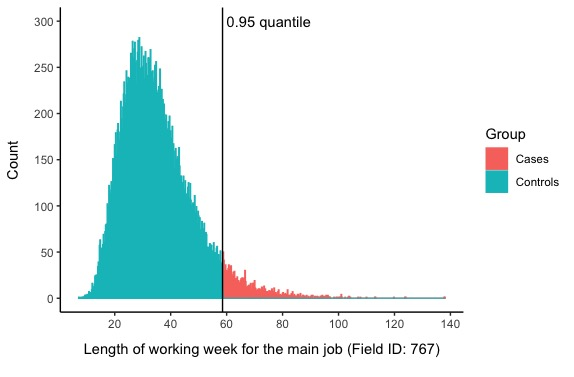
\includegraphics[width=500px]{/Users/munchausend/GoogleDrive/Git/raeBiobank/PR/Plots/PopOfInterest} \caption{\emph{Defining our population of interest. We will take the top 5\% of the sample distribution (n = 35,501) for `Length of working week for the main job' (Biobank Field ID: 767) to represent our population of interest (i.e.~`Cases'; n = 1,775), and select matched case-controls (i.e.~`Controls'; n = 1,775) from the remainder of the sample (n = 33,726). The above is an illustration of this procedure, using a simulated distribution for n = 35,501, based on estimates available from the data provider (\url{https://biobank.ctsu.ox.ac.uk/crystal/field.cgi?id=767}). Code available at \url{https://github.com/factitious/raeBiobank_workingBrain/tree/master/PR/Plots/Histo.R}}}\label{fig:figure}
\end{figure}

Next, we will find a set of matched controls from the remaining 95\% of the sample who work fewer hours. We aim to identify a group of \textasciitilde1,775 subjects who work fewer hours than the case group, but who are matched on key sociodemographic, lifestyle and environment, and health-related characteristics (see \textbf{Identifying matching variables}).

Once we have completed our case-control analysis of neuroimaging, immunological, and cognitive markers for `\emph{Length of working week for main job}', we will seek to repeat the process for other potentially deleterious occupational factors (such as commute time or shift work). These subsequent analyses will likely identify a different set of \textasciitilde1,775 cases and \textasciitilde1,755 controls, although some individuals may be present across multiple analyses.

\textbf{Identifying matching variables}. To determine the variables that need to be included in the matching process, we will compare the 5\% case group of interest to the remaining 95\% of the sample on all Data Fields in our project 62188 dataset (see \url{http://tiny.cc/UKBBMetaData_62188}), excluding the occupational factor of interest that defines the status of the 5\% case group, and the neuroimaging, immunological, and cognitive variables of interest. We plan to use the following methods:

\begin{itemize}
\item
  \emph{Test statistics} (e.g.~t-test, chi-square) comparing the population of interest with the 95\% rest of the sample on all the possible matching variables. Variables with a Family Discovery Rate (FDR) adjusted p-value lower than a pre-defined cut-off point (p\textless0.05) would be selected for matching. If this generates a very large number of matching variables with the consequence that it is impossible to identify at least \textasciitilde1,775 matched controls, we will take the variables with the most significant p-values to match on, progressively adding in further variables until we can no longer identify a minimum of \textasciitilde1,775 control individuals.
\item
  \emph{Random forests}, a classifier approach to identifying the most important features that characterise a dataset. This approach will be applied to estimate variable importance measures (e.g.~permutation importance), which will tell us how much each variable contributes to the characterisation of an individual as working long hours, and therefore, how important it is to match on this variable. All relevant variables, as determined by the selected importance scores, would be selected for matching. As with the \emph{test statistics} approach, if this generates a very large number of matching variables with the consequence that it is impossible to identify at least \textasciitilde1,775 matched controls, we will take the variables with the largest importance values to match on, progressively adding in further variables until we can no longer identify a minimum of \textasciitilde1,775 control individuals.
  We plan to run both the \emph{test statistics} and \emph{random forests} feature selection approaches to gain an overview of consistency between the two methods (i.e., if the same features appear as important to match cases and controls on, across the two approaches, this gives additional confidence).
\item
  \emph{Other means of identifying matching variables} may evolve as we proceed through the descriptive stages of the analysis, and will be recounted in successive updates to this present preregistration document.
\end{itemize}

\textbf{Case-control matching}. After determining the variables to include in the matching process, appropriate distance measures will be determined for each variable (e.g.~propensity scores), and a matching method implemented (e.g.~nearest neighbour).

\newpage

\hypertarget{multistage-preregistration-plan}{%
\subsection{Multistage preregistration plan}\label{multistage-preregistration-plan}}

We intend to successively update our preregistration documentation as we proceed through each analysis step in this project. This document (dated October 20th, 2020) forms the second document in this series. As we complete data analysis stages, we will be able to prescribe increasingly specific hypotheses, and refine our original broad imaging and physiological analysis approaches set out in earlier preregistration documentation, to increasingly more precise plans. This will include an evolution of expected statistical approaches as the multifactorial complexities of our dataset reveal themselves in relation to our specific questions about brain, body and behavioural markers of occupational wellbeing.

We will seek to timestamp our data logs and analysis records and provide updated pre-gregistration documents in a public repository, such that the evolutionary timeline is indicative of a commitment to preregistration principles, (i.e.~to guard against questionable research practices) while taking account of the multi-stage and complex nature of this project.

\newpage

\newpage

\hspace{1cm}

\hypertarget{refs}{}
\begin{cslreferences}
\leavevmode\hypertarget{ref-TUC1}{}%
1. TUC. (2019). British workers putting in longest hours in the EU, TUC analysis finds. Retrieved from \url{https://www.tuc.org.uk/news/british-workers-putting-longest-hours-eu-tuc-analysis-finds}

\leavevmode\hypertarget{ref-TUC2}{}%
2. TUC. (2019). Annual commuting time is up 21 hours compared to a decade ago, finds TUC. Retrieved from \url{https://www.tuc.org.uk/news/annual-commuting-time-21-hours-compared-decade-ago-finds-tuc}

\leavevmode\hypertarget{ref-TotallyMoney}{}%
3. TotallyMoney. (2019). Overtime Survey 2018 - how much overtime does the UK work? Retrieved from \url{https://www.totallymoney.com/overtime-survey/}

\leavevmode\hypertarget{ref-Bannai2014}{}%
4. Bannai, A., \& Tamakoshi, A. (2014). The association between long working hours and health: A systematic review of epidemiological evidence. \emph{Scandinavian Journal of Work, Environment \& Health}, \emph{40}(1), 5--18. \url{http://dx.doi.org/10.5271/sjweh.3388}

\leavevmode\hypertarget{ref-Kim2016}{}%
5. Kim, W., Park, E. C., Lee, T. H., \& Kim, T. H. (2016). Effect of working hours and precarious employment on depressive symptoms in South Korean employees: A longitudinal study. \emph{Occupational and Environmental Medicine}, \emph{73}(12), 816--822. \url{http://dx.doi.org/10.1136/oemed-2016-103553}

\leavevmode\hypertarget{ref-Kajitani2018}{}%
6. Kajitani, S., McKenzie, C., \& Sakata, K. (2018). Use It Too Much and Lose It? The Effect of Working Hours on Cognitive Ability. \emph{SSRN Electronic Journal}. \url{http://dx.doi.org/10.2139/ssrn.2737742}

\leavevmode\hypertarget{ref-VanderHulst2003}{}%
7. Hulst, M. van der. (2003). Long workhours and health. Finnish Institute of Occupational Health. \url{http://dx.doi.org/10.5271/sjweh.720}

\leavevmode\hypertarget{ref-Akerstedt2001}{}%
8. Akerstedt, T., Olsson, B., Ingre, M., Holmgren, M., \& Kecklund, G. (2001). \emph{A 6-hour working day--effects on health and well-being.} (Vol. 30, pp. 197--202). \url{http://dx.doi.org/10.11183/jhe1972.30.197}

\leavevmode\hypertarget{ref-Barck-Holst2017}{}%
9. Barck-Holst, P., Institutet, K., Åkerstedt, S. T., Hellgren, C., Nilsonne, Å., Åkerstedt, T., \ldots{} Hellgren, C. (2017). Reduced working hours and stress in the Swedish social services: A longitudinal study. \emph{International Social Work}, \emph{60}(4), 897--913. \url{http://dx.doi.org/10.1177/0020872815580045}

\leavevmode\hypertarget{ref-Basner2014}{}%
10. Basner, M., Spaeth, A. M., \& Dinges, D. F. (2014). Sociodemographic Characteristics and Waking Activities and their Role in the Timing and Duration of Sleep. \emph{Sleep}, \emph{37}(12), 1889--1906. \url{http://dx.doi.org/10.5665/sleep.4238}

\leavevmode\hypertarget{ref-Basner2018}{}%
11. Basner, M., Dinges, D. F., \& Basner, M. (2018). Ac c te d us cr ip t pt cr t. \emph{Sleep}, \emph{41}(4), zsy012. \url{http://dx.doi.org/10.1093/sleep/zsy012/4792945}

\leavevmode\hypertarget{ref-Simpson2016}{}%
12. Simpson, N. S., Diolombi, M., Scott-Sutherland, J., Yang, H., Bhatt, V., Gautam, S., \ldots{} Haack, M. (2016). Repeating patterns of sleep restriction and recovery: Do we get used to it? \emph{Brain, Behavior, and Immunity}, \emph{58}, 142--151. \url{http://dx.doi.org/10.1016/j.bbi.2016.06.001}

\leavevmode\hypertarget{ref-Reinhardt2016}{}%
13. Reinhardt, É. L., Fernandes, P. A. C. M. C. M., Markus, R. P., \& Fischer, F. M. (2016). Short sleep duration increases salivary IL-6 production. \emph{Chronobiology International}, \emph{33}(6), 780--782. \url{http://dx.doi.org/10.3109/07420528.2016.1167710}

\leavevmode\hypertarget{ref-Buxton2010}{}%
14. Buxton, O. M., Pavlova, M., Reid, E. W., Wang, W., Simonson, D. C., \& Adler, G. K. (2010). Sleep restriction for 1 week reduces insulin sensitivity in healthy men. \emph{Diabetes}, \emph{59}(9), 2126--2133. \url{http://dx.doi.org/10.2337/db09-0699}

\leavevmode\hypertarget{ref-Marucci-Wellman2016}{}%
15. Marucci-Wellman, H. R., Lombardi, D. A., \& Willetts, J. L. (2016). Chronobiology International The Journal of Biological and Medical Rhythm Research Working multiple jobs over a day or a week: Short-term effects on sleep duration. \url{http://dx.doi.org/10.3109/07420528.2016.1167717}

\leavevmode\hypertarget{ref-Howren2009}{}%
16. Howren, M. B., Lamkin, D. M., \& Suls, J. (2009). Associations of depression with c-reactive protein, IL-1, and IL-6: A meta-analysis. \emph{Psychosomatic Medicine}, \emph{71}(2), 171--186. \url{http://dx.doi.org/10.1097/PSY.0b013e3181907c1b}

\leavevmode\hypertarget{ref-Critchley2013}{}%
17. Critchley, H. D., \& Harrison, N. A. (2013, February). Visceral Influences on Brain and Behavior. Cell Press. \url{http://dx.doi.org/10.1016/j.neuron.2013.02.008}

\leavevmode\hypertarget{ref-Critchley2017}{}%
18. Critchley, H. D., \& Garfinkel, S. N. (2017). Interoception and emotion. \emph{Current Opinion in Psychology}, \emph{17}, 7--14. \url{http://dx.doi.org/10.1016/j.copsyc.2017.04.020}

\leavevmode\hypertarget{ref-Rae2018}{}%
19. Rae, C., Botan, V. E., Gould Van Praag, C. D., Herman, A. M., Nyyssönen, J. A. K., Watson, D. R., \ldots{} Critchley, H. D. (2018). Response inhibition on the stop signal task improves during cardiac contraction. \emph{Scientific Reports}, \emph{8}(1). \url{http://dx.doi.org/10.1038/s41598-018-27513-y}

\leavevmode\hypertarget{ref-Yoo2007a}{}%
20. Yoo, S. S., Gujar, N., Hu, P., Jolesz, F. A., \& Walker, M. P. (2007, October). The human emotional brain without sleep - a prefrontal amygdala disconnect. Elsevier. \url{http://dx.doi.org/10.1016/j.cub.2007.08.007}

\leavevmode\hypertarget{ref-Motomura2014}{}%
21. Motomura, Y., Kitamura, S., Oba, K., Terasawa, Y., Enomoto, M., Katayose, Y., \ldots{} Mishima, K. (2014). \emph{Sleepiness induced by sleep-debt enhanced amygdala activity for subliminal signals of fear}. \url{http://dx.doi.org/10.1186/1471-2202-15-97}

\leavevmode\hypertarget{ref-Motomura2013}{}%
22. Motomura, Y., Kitamura, S., Oba, K., Terasawa, Y., Enomoto, M., Katayose, Y., \ldots{} Mishima, K. (2013). Sleep Debt Elicits Negative Emotional Reaction through Diminished Amygdala-Anterior Cingulate Functional Connectivity. \emph{PLoS ONE}, \emph{8}(2), e56578. \url{http://dx.doi.org/10.1371/journal.pone.0056578}

\leavevmode\hypertarget{ref-Prather2013}{}%
23. Prather, A. A., Bogdan, R., \& Hariri, A. R. (2013). Impact of sleep quality on amygdala reactivity, negative affect, and perceived stress. \emph{Psychosomatic Medicine}, \emph{75}(4), 350--358. \url{http://dx.doi.org/10.1097/PSY.0b013e31828ef15b}

\leavevmode\hypertarget{ref-Zhao2018}{}%
24. Zhao, R., Zhang, X., Fei, N., Zhu, Y., Sun, J., Liu, P., \ldots{} Qin, W. (2018). Decreased cortical and subcortical response to inhibition control after sleep deprivation. \emph{Brain Imaging and Behavior}, \emph{13}(3), 638--650. \url{http://dx.doi.org/10.1007/s11682-018-9868-2}

\leavevmode\hypertarget{ref-Cui2015}{}%
25. Cui, J., Tkachenko, O., Gogel, H., Kipman, M., Preer, L. A., Weber, M., \ldots{} Killgore, W. D. S. (2015). Microstructure of frontoparietal connections predicts individual resistance to sleep deprivation. \emph{NeuroImage}, \emph{106}, 123--133. \url{http://dx.doi.org/10.1016/j.neuroimage.2014.11.035}

\leavevmode\hypertarget{ref-Krause2017}{}%
26. Krause, A. J., Simon, E. B., Mander, B. A., Greer, S. M., Saletin, J. M., Goldstein-Piekarski, A. N., \& Walker, M. P. (2017, July). The sleep-deprived human brain. Nature Publishing Group. \url{http://dx.doi.org/10.1038/nrn.2017.55}

\leavevmode\hypertarget{ref-Ma2015}{}%
27. Ma, N., Dinges, D. F., Basner, M., \& Rao, H. (2015). How Acute Total Sleep Loss Affects the Attending Brain: A Meta-Analysis of Neuroimaging Studies. \emph{Sleep}, \emph{38}(2), 233--240. \url{http://dx.doi.org/10.5665/sleep.4404}

\leavevmode\hypertarget{ref-Hariri2002a}{}%
28. Hariri, A. R., Tessitore, A., Mattay, V. S., Fera, F., \& Weinberger, D. R. (2002). The amygdala response to emotional stimuli: A comparison of faces and scenes. \emph{NeuroImage}, \emph{17}(1), 317--323. \url{http://dx.doi.org/10.1006/nimg.2002.1179}

\leavevmode\hypertarget{ref-Sudlow2015}{}%
29. Sudlow, C., Gallacher, J., Allen, N., Beral, V., Burton, P., Danesh, J., \ldots{} Collins, R. (2015). UK Biobank: An Open Access Resource for Identifying the Causes of a Wide Range of Complex Diseases of Middle and Old Age. \emph{PLoS Medicine}, \emph{12}(3). \url{http://dx.doi.org/10.1371/journal.pmed.1001779}

\leavevmode\hypertarget{ref-Yeo2015}{}%
30. Yeo, B. T., Tandi, J., \& Chee, M. W. L. (2015). Functional connectivity during rested wakefulness predicts vulnerability to sleep deprivation. \emph{NeuroImage}, \emph{111}, 147--158. \url{http://dx.doi.org/10.1016/j.neuroimage.2015.02.018}

\leavevmode\hypertarget{ref-DeHavas2012}{}%
31. De Havas, J. A., Parimal, S., Soon, C. S., \& Chee, M. W. L. (2012). Sleep deprivation reduces default mode network connectivity and anti-correlation during rest and task performance. \emph{NeuroImage}, \emph{59}(2), 1745--1751. \url{http://dx.doi.org/10.1016/j.neuroimage.2011.08.026}

\leavevmode\hypertarget{ref-Shao2014}{}%
32. Shao, Y., Lei, Y., Wang, L., Zhai, T., Jin, X., Ni, W., \ldots{} Yang, Z. (2014). Altered Resting-State Amygdala Functional Connectivity after 36 Hours of Total Sleep Deprivation. \emph{PLoS ONE}, \emph{9}(11), e112222. \url{http://dx.doi.org/10.1371/journal.pone.0112222}

\leavevmode\hypertarget{ref-Lei2015}{}%
33. Lei, Y., Shao, Y., Wang, L., Ye, E., Jin, X., Zou, F., \ldots{} Yang, Z. (2015). Altered superficial amygdala-cortical functional link in resting state after 36 hours of total sleep deprivation. \emph{Journal of Neuroscience Research}, \emph{93}(12), 1795--1803. \url{http://dx.doi.org/10.1002/jnr.23601}

\leavevmode\hypertarget{ref-Samann2010}{}%
34. Sämann, P. G., Tully, C., Spoormaker, V. I., Wetter, T. C., Holsboer, F., Wehrle, R., \& Czisch, M. (2010). Increased sleep pressure reduces resting state functional connectivity. \emph{Magnetic Resonance Materials in Physics, Biology and Medicine}, \emph{23}(5-6), 375--389. \url{http://dx.doi.org/10.1007/s10334-010-0213-z}

\leavevmode\hypertarget{ref-Meier-Ewert2004}{}%
35. Meier-Ewert, H. K., Ridker, P. M., Rifai, N., Regan, M. M., Price, N. J., Dinges, D. F., \& Mullington, J. M. (2004). Effect of sleep loss on C-Reactive protein, an inflammatory marker of cardiovascular risk. \emph{Journal of the American College of Cardiology}, \emph{43}(4), 678--683. \url{http://dx.doi.org/10.1016/j.jacc.2003.07.050}

\leavevmode\hypertarget{ref-Schiller2018}{}%
36. Schiller, H., Lekander, M., Rajaleid, K., Hellgren, C., Åkerstedt, T., Barck-Holst, P., \& Kecklund, G. (2018). Total workload and recovery in relation to worktime reduction: A randomised controlled intervention study with time-use data. \emph{Occupational and Environmental Medicine}, \emph{75}(3), 218--226. \url{http://dx.doi.org/10.1136/oemed-2017-104592}
\end{cslreferences}

\end{document}
